\documentclass[11pt]{article}
%Gummi|065|=)
\usepackage[utf8]{inputenc}
\usepackage{cite}
\usepackage{mathtools}
\usepackage{multirow}
\usepackage{chngpage}



\title{\textbf{Shared memory vs Distributed memory}}
\author{Cengiz Önkal\\21706071}
\date{}

\usepackage{graphicx}
\begin{document}

\maketitle

\begin{abstract}
This paper discusses and compares Shared Memory structure to Distributed Memory structure.
\end{abstract}




\section{Introduction}
Shared memory systems form a major category of multiprocessors. In this category,
all processors share a global memory. Communication between tasks running on
different processors is performed through writing to and reading from the global
memory. All interprocessor coordination and synchronization is also accomplished
via the global memory
On the other hand \textbf{distributed memory} refers to a multiprocessor computer system in which each processor (CPU) has its own private memory.

\section{Shared Memory}
The simplest shared memory system consists of one memory module that can be accessed from two processors. Requests arrive at the memory module through its two ports. An arbitration unit within the memory
module passes requests through to a memory controller. If the memory module is
not busy and a single request arrives, then the arbitration unit passes that request
to the memory controller and the request is satisfied. The module is placed in the
busy state while a request is being serviced. If a new request arrives while the
memory is busy servicing a previous request, the memory module sends a wait
signal, through the memory controller, to the processor making the new request.
In response, the requesting processor may hold its request on the line until the
memory becomes free or it may repeat its request some time later.\cite{el2005advanced} 


Two main problems need to be addressed when designing a shared memory
system: performance degradation due to conflict, and coherence problems. Performance degradation might happen when multiple processors are trying to access the shared memory simultaneously. A typical design might use caches to solve the contention problem. However, having multiple copies of data, spread throughout the caches, might lead to a coherence problem. 

Based on the interconnection network used, shared
memory systems can be categorized in the following categories.

\subsection{Uniform Memory Access (UMA)}
In the UMA system a shared memory is accessible by all processors through an
interconnection network in the same way a single processor accesses its memory.
All processors have equal access time to any memory location. The interconnection
network used in the UMA can be a single bus, multiple buses, or a crossbar switch.
Because access to shared memory is balanced, these systems are also called SMP
(symmetric multiprocessor) systems. Each processor has equal opportunity to
read/write to memory, including equal access speed. Commercial examples of
SMPs are \textbf{Sun Microsystems multiprocessor servers} and \textbf{Silicon Graphics Inc. multiprocessor servers}.
\begin{figure}[htp]
\centering
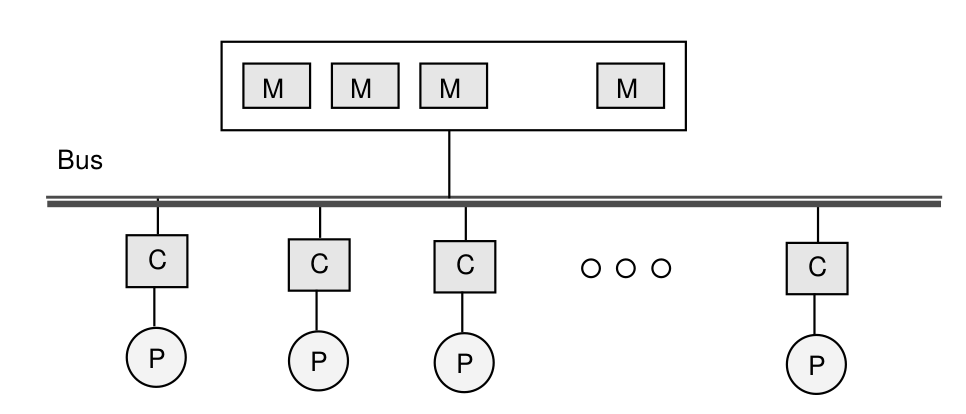
\includegraphics[scale=0.30]{uma.png}
\caption{Uniform Memory Access}
\end{figure}

% subsection  (end)
\subsection{Nonuniform Memory Access (NUMA)}
In the NUMA system a, each processor has a part of shared memory. The shared memory has a single adress space. This means each processor can access any memory location directly using its real address. However, the access time to modules depends on the distance to the processor.Beacuse of this memory access time is not uniform. \textbf{SGI Origin 3000} can be given as example for this architecture.


\begin{figure}[htp]
\centering
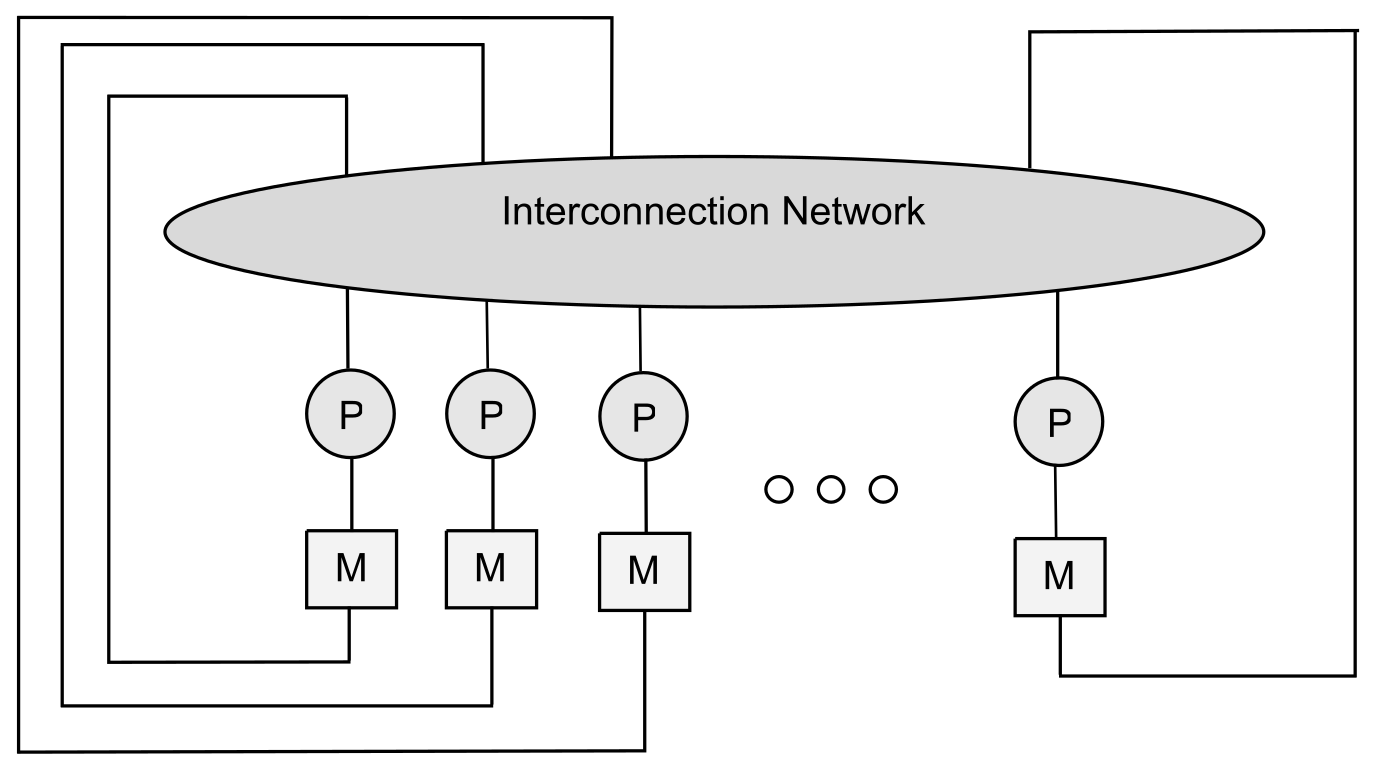
\includegraphics[scale=0.20]{numa.png}
\caption{Nonuniform Memory Access}
\end{figure}
% subsection  (end)


\subsection{Cache-Only Memory Architecture (COMA)}
In this system each processor has part of the shared memory like in the NUMA.
However, in this case the shared memory consists of cache memory. A COMA
system requires that data be migrated to the processor requesting it. There is no memory hierarchy and the address space is made of all the caches. There is a cache directory (D) that helps in remote cache access. The Kendall Square Research’s \textbf{KSR-1} machine is an example of such architecture.
% subsection (end)



\subsection{Shared Memory Programming}
Shared memory parallel programming is perhaps the easiest model to understand
because of its similarity with operating systems programming and general multiprogramming. Shared memory programming is done through some extensions to existing programming languages, operating systems, and code libraries.


\section{Distributed Memory}
Distributed Memory systems provide alternative methods for communication and
movement of data among multiprocessors (compared to shared memory multiprocessor systems). A message passing system typically combines local memory and the processor at each node of the interconnection network. There is no global memory so it is necessary to move data from one local memory to another by means of message passing. This is typically done by send/receive pairs of commands, which must be written into the application software by a programmer.

The basis for the scheme is that each processor has its own local memory and communicates with other processors using messages. The elimination of the need for a large global memory together with its synchronization requirement, gives message passing schemes an edge over shared memory schemes.

\begin{figure}[htp]
\centering
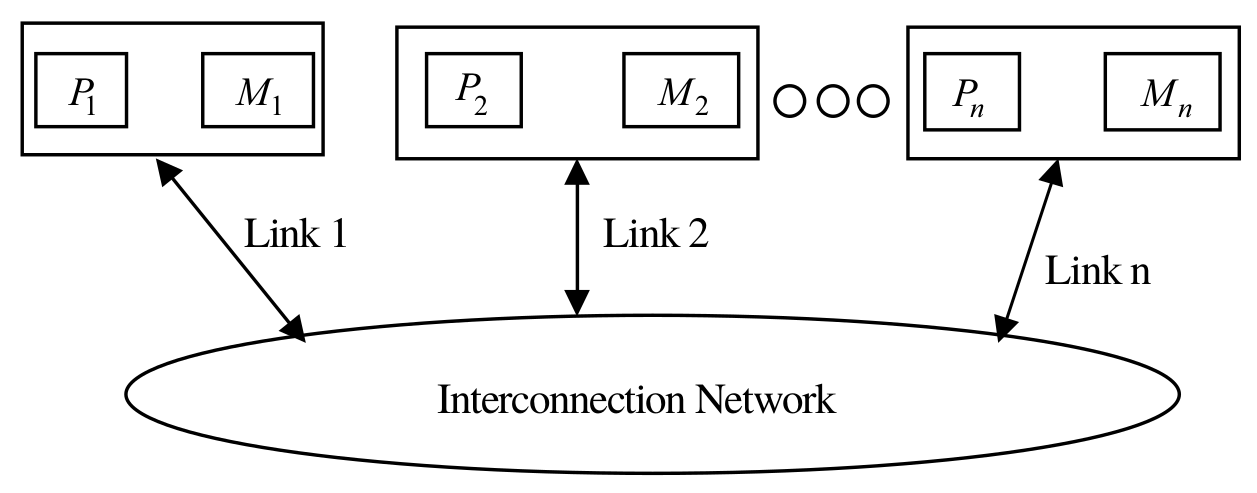
\includegraphics[scale=0.25]{distributed.png}
\caption{Distributed Memory}
\end{figure}

Process Granularity The size of a process in a distributed memory system can be described by a parameter called process granularity. This is defined as follows.

\begin{equation}
 \textbf{Process Granularity}= \frac{\text{computation time}}  {\text{communication time}}
\end{equation}

 
\begin{itemize}
  \item Coarse granularity: Each process holds a large number of sequential instructions and takes a substantial amount of time to execute.
  \item Medium granularity: Since the process communication overhead increases as the granularity decreases, medium granularity describes a middle ground
where communication overhead is reduced.
  \item Fine granularity: Each process contains a few sequential instructions (as few
as just one instruction).
\end{itemize}



\subsection{Routing}
Routing is defined as the techniques used for a message to select a path over the network channels.
Two important factors must be considered in designing distributed systems interconnection networks: link bandwidth and the network latency.The link bandwidth is defined as the number of bits that can be transmitted per unit of time (bits/s). Network latency is defined as the time to complete a message transfer through the network.There are two types of communication operation in distributed systems, which are one-to-one (\textit{unicast}) and \textit{collective} communications. Boardcast and multicast are the most widely used in collective communications.

A number of possible problems can result from the use of certain routing mechan-
isms in message passing systems.

\begin{itemize}
\item{Deadlock: When two messages each hold the resources required by the other in
order to move, both messages will be blocked}
\item{Livelock:a situation in which a message keeps going around
the network and never reaches its destination.}

\item{Starvation: A node is said to suffer from starvation if it has a message to inject into the network but is never allowed to do so.}
\end{itemize}


\subsection{Switching Mechanisms}
Switching mechanisms refer to the mechanisms used to remove data from an input channel and place it on an output channel. Network latency is highly dependent on the switching mechanism used.
Some of the switching mechanisms are;
\begin{itemize}
\item{\textbf{circuit-switching networks}: the path between the source and destination is first determined, all links along that path are reserved, and no buffers are needed in each node. After data transfer, reserved links are released for use by other messages}
\item{\textbf{store-and-forward switching mechanism} is to offer dynamic bandwidth allocation to messages as they flow through the network, to avoid the main drawback of the circuit-
switching mechanism.}
\item{\textbf{packet-switched}}
\item{\textbf{virtual cut-through}}
\end{itemize}

\begin{adjustwidth}{-1in}{-1in} 
\begin{center}
\begin{tabular}{ |l|l|l| } 
\hline
 Switching Mechanism & Advantages & Disadvantages \\ 
\hline
\multirow{2}{8em}{Circuit switching} & Suitable for long messages & Wasting of bandwidth \\ & Deadlock-free & \\ 
\hline
\multirow{3}{8em}{Store and forward} & Simple & Buffer for every packet  \\
& Suitable for interactive traffic & Potential long latency \\ 
& Bandwidth on demand & Potential deadlock \\ 
\hline
\multirow{3}{8em}{Virtual cut-through} & Good for long messages & Need for multiple message
buffers  \\
& Possible deadlock avoidance & Wasting of bandwidth \\ 
& Elimination of data-link
protocol & Mainly used with
profitable routing \\ 
\hline
\end{tabular}
\end{center}
\end{adjustwidth}

\subsection{Distributed Memory Programming Models}
This architecture uses a set of commands that allows processes to
communicate with each other. These include the send, receive, broadcast, and barrier
commands. The send command takes a memory buffer and sends it to a destination
node. The receive command accepts a message from a source node and stores it in a
specified memory buffer. The basic programming model used in distributed memory architectures is based on the idea of matching a send request on one processor with a receive request on another. 
In such scheme, send and receive are blocking; that is, send blocks until the corresponding receive is executed before data can be transferred.


%subsection (end)


\section{Distributed Memory vs Shared Memory}

In the shared-memory architecture all the CPU cores can access the same memory and are all controlled by a single operating system. Modern processors are all multicore processors, with many CPU-cores manufactured together on the same physical silicon chip.With this shared memory enjoys the desirable feature that all
communications are done using implicit loads and stores to a global address space.

There are, however, limitations to the shared-memory approach due to all the CPU-cores competing for access to memory over a shared bus, much like the obvious issues in trying to cram too many workers into the same office. This can be alleviated to some extent by introducing memory caches or putting several processors together in a NUMA architecture, but there is no way we can reach the hundreds of thousands of CPU-cores we need for today’s multi-petaflop supercomputers.

Shared memory systems may be easier to program, but are difficult to scale up to a large number of processors. If scalability to larger and larger systems (as measured by the number of processing units) was to continue, systems had to use distributed memory techniques. It is apparent that message passing systems are the only way to efficiently increase the number of processors managed by a multiprocessor system.
There are, however, a number of problems associated with message passing systems.
These include communication overhead and difficulty of programming.

\bibliographystyle{plain}
\bibliography{references}


\end{document}
